\documentclass[brazil,12p,A4]{abnt}
\usepackage{paralist}
\usepackage{graphicx,url,subfigure}
\usepackage[brazil]{babel}
\usepackage[utf8]{inputenc}
\usepackage[T1]{fontenc}
\usepackage{ae}
\usepackage[alf,bibjustif,abnt-etal-list=0]{abntcite}
\usepackage{alltt}
\usepackage{booktabs}
\usepackage{float}
\usepackage{amssymb}
\usepackage{amsmath}

\usepackage[nice]{nicefrac}

\usepackage{rotating}
\usepackage{multirow}

\usepackage{color}
\usepackage{caption}
\usepackage{listings}
\lstset{
  basicstyle=\footnotesize\ttfamily,
  stepnumber=1,
  numbersep=5pt,
  tabsize=2,
  extendedchars=true,
  breaklines=true,
  keywordstyle=\bfseries,
  showspaces=false,
  showtabs=false,
  xleftmargin=17pt,
  framexleftmargin=17pt,
  framexrightmargin=5pt,
  framexbottommargin=4pt,
  showstringspaces=false,
}
\lstloadlanguages{
  C
}

\DeclareCaptionFont{black}{\color{black}}
\DeclareCaptionFormat{listing}{#1#2#3}
\captionsetup[lstlisting]{format=listing, textfont=black,
  }

\newfloat{model}{thp}{lop}
%\captionof{model}{Modelo}
\floatname{model}{Modelo}

\newcommand{\up}[1]{\raisebox{1.5ex}[0pt]{#1}}
\newcommand{\doctitulo}{Bitcity}
\newcommand{\docautor}{Guilherme Enoc Egas\\Guilherme Henrique Polo Gonçalves\\
	Maycon Sambinelli}

\renewcommand{\lstlistingname}{Algoritmo}
\renewcommand{\lstlistlistingname}{Algoritmo}


\begin{document}

\baselineskip=.7cm


\vspace{4cm}

\begin{center}

\textbf{UNIVERSIDADE ESTADUAL DE MARINGÁ}

\textbf{CENTRO DE TECNOLOGIA}

\textbf{DEPARTAMENTO DE INFORMÁTICA}

\vspace{4cm}

\textbf{\MakeUppercase{\doctitulo}}

\vspace{1cm}

%\MakeUppercase{\docautor}
\docautor

\vspace{1cm}

\end{center}

\vspace{10cm}

\begin{center}
\centering
\textbf{Maringá - Paraná}

\textbf{2010}
\end{center}


\pagebreak

{
\Large
\begin{center}
\textbf{Resumo}
\end{center}
}

Concorrência é quando duas ou mais unidades são executadas em simultâneo. Como estas unidades
podem compartilhar os mesmo recursos, isto pode acarretar em alguns problemas: condição de
corrida e deadlock. Assim, para evitar estes problemas, se torna necessário encontrar uma forma
de sincronizar as unidades, consequentemente mantendo consistência nas informações utilizadas.
Erros são comuns em tempo de execução e as aplicações devem estar preparadas para lidar com eles.
Com o uso de exceções, podemos interromper o fluxo normal do programa quando ocorrer um erro e, assim,
podemos trata-lo sem precisar abortar a execução do programa.

\quad\\
\quad\\
\textit{Palavras-chave}: Concorrência, Exceções, Java

\pagebreak


\tableofcontents


\pagebreak

\chapter{Introdução}

Alguns problemas possuem uma solução concorrente mais natural do que a
sequencial, é o caso de muitos problemas de simulação, onde diversas
variáveis do problema são modificadas independentemente e de forma
concorrente. É o caso da simulação de uma cidade, um carro $i$ não se move
para depois um carro $j$ se mover, eles se movem de forma independente um
do outro.

Além de ser a solução mais natural para alguns tipos de problema, muitos
computadores atualmente possuem múltiplos processadores e, dessa forma, 
uma aplicação pode aumentar sua performance usando a concorrência em tais
arquiteturas.

Outro recurso importante que muitas linguagens modernas implementam é o
tratamento de exceções. Uma exceção é qualquer evento errôneo, ou não,
que seja detectável por \textit{hardware} ou \textit{software} e que possa
exigir processamento especial \cite{sebesta}. O suporte de exceções pela
linguagem aumenta a confiabilidade do programa e força o programador
a desenvolver pensando nos casos extremos.

Este trabalho está dividido da forma seguinte. No Capítulo
\ref{cha:concexec} é feita uma pequena introdução a concorrência, seus
principais problemas, seus mecanismos de sincronização e exceções. O
Capítulo \ref{cha:concjava} aborda os principais mecanismos oferecidos pela
linguagem Java para implementar a concorrência e manipular exceções. O
Capítulo \ref{cha:bitcity} apresenta um simulador de uma cidade que faz
uso dos mecanismo de concorrência, sincronização e tratamento de
exceções em Java. No Capítulo \ref{cha:conclusao} é apresentada as
vantagens e desvantagens do suporte pela linguagem a concorrência e
exceções. 

\chapter{Concorrência e Exceções}

Há alguns níveis de concorrência: concorrência de instrução de máquina, onde são
executadas mais do que uma instrução de máquina por vez; concorrência de
instrução, onde são executadas mais do que uma instrução por vez;
concorrência em nível de unidade, onde são executadas mais do que uma
unidade de subprograma por vez; nível de programa, onde são executados mais
do que um subprograma por vez. 

Uma unidade pode ser executada concorrentemente de duas formas: fisicamente
ou logicamente. Na concorrência física duas ou mais unidades do mesmo
programa são executadas simultaneamente, sendo necessário a existência de
mais de um processador para que isso seja possível. Quando não há a
disponibilidade de múltiplos processadores pode ocorrer a concorrência
lógica, onde o programador e o programa supõem a existência de múltiplos
processadores fornecendo a concorrência física, enquanto na verdade a
execução das unidades está sendo realizada de forma intercalada. Esta
ilusão é semelhante à ilusão de execução simultânea oferecida a diferentes
usuários de um sistema de computadores com multiprogramação.

Para visualizar um fluxo de execução de um programa, podemos imaginar uma
linha ({\it thread}) disposta sobre o código fonte. Cada linha representa um
fluxo de execução dentro do programa. Programas executando em computadores
multiprocessadores podem executar cada fluxo (linha) em um processador
diferente simultaneamente. Na concorrência lógica,  múltiplas linhas do
programa são mapeadas em apenas uma, fazendo com que o programa tenha
virtualmente múltiplas linhas. 

Uma tarefa é uma unidade de um programa que pode estar em execução
concorrente com outras unidades do mesmo programa. Cada tarefa de um
programa pode oferecer uma linha de controle \cite{sebesta}. Diferente de
um subprograma, as tarefas podem ser implicitamente inicializadas e, além
disso, quando uma unidade invoca uma tarefa, ela não precisa esperar que
está termine para continuar a sua execução.

Como todas as linhas compartilham os mesmos dados é necessário a utilização
de algum mecanismo de sincronização para manter a consistência desses
dados. Atualmente o método de se fazer sincronização mais utilizada é
a exclusão mútua \cite{ARTOFMPP, MCRT}. 

Este Capítulo está organizado da seguinte maneira: Na Seção \ref{sub:prob}
será abordado alguns problema comuns na programação paralela. A Seção
\ref{sub:mecanismo} abordará alguns mecanismos utilizados para se fazer
a sincronização. Por último, a Seção \ref{sub:except} apresenta 
conceitos a cerca das exceções.

\section{Problemas Comuns na Computação Paralela}
\label{sub:prob}

\subsection{Condição de Corrida}

Quando duas tarefas trabalham juntas, eles podem compartilhar algum recurso
em comum. Uma condição de corrida ocorre quando duas ou mais tarefas
necessitam efetuar operações em um conjunto de dados compartilhado e o 
resultado destas operações dependem da ordem em que essas operações
são executadas \cite{tanen}.

\subsection{Deadlock}

Um conjunto de tarefas estará em situação de \textit{deadlock} se todas as
tarefas pertencentes ao conjunto estiverem esperando por um evento que somente
tarefa desse mesmo conjunto possa realizar. Como todas as tarefas estarão
esperando, nenhuma delas desencadeará qualquer um dos eventos que a outra
esta esperando e, assim, todas as atividades continuam a esperar para sempre.

Para que ocorra um \textit{Deadlock}, deve haver quatro condições satisfeitas:

\begin{itemize}
\item \textit{Condição de exclusão mútua}: Em um determinado instante,
cada recurso está em uma de duas situações: ou associado a uma única tarefa
ou disponível. 
\item \textit{Condição de posse e espera}: Tarefas que,
em um determinado instante, retêm recursos concedidos anteriormente podem
requisitar novos recursos. 
\item \textit{Condição de não preempção}:
Recursos concedidos previamente a uma tarefa não podem ser forçadamente
tomados - eles deve ser explicitamente liberados pela tarefa que os retém.
\item \textit{Condição de espera circular}: Deve existir um encadeamento
circular de duas ou mais tarefas; cada uma delas encontra-se à espera de
um recurso que está sendo usado pelo membro seguinte dessa cadeia.
\end{itemize}

Todas essas quatro condições deve estar presentes para que um
\textit{deadlock} ocorra. Se faltar uma delas, não ocorrerá
\textit{deadlock}.

Em geral, quatro estratégias são usadas para tratar \textit{deadlocks}:

\begin{itemize}
\item Ignorar por completo o problema.
\item Detecção e recuperação. Deixar os \textit{deadlocks} ocorrer,
detectá-los e agir.
\item Anulação dinâmica por meio de uma alocação cuidadosa de recursos.
\item Prevenção, negando estruturalmente algumas das condições necessárias
para gerar um \textit{deadlock}.
\end{itemize}

%\subsubsection{Livelock}
%
% WTF?
%Um \textit{Livelock} é semelhante a um \textit{Deadlock}, com exceção dos estados dos processos envolvidos na 
%\textit{Livelock} mudam constantemente em relação um ao outro, nenhum progresso \textit{Livelock} é um caso 
%especial de esgotamento de recursos.
%
%Um exemplo do mundo real de \textit{Livelock} ocorre quando duas pessoas se encontram em um corredor 
%estreito, e cada um tenta ser educada, movendo de lado para  dar passagem a outra pessoa, 
%mas eles acabam movendo de um lado para o outro sem fazer nenhum progresso porque ambos 
%repetidamente movem na mesma direção e ao mesmo tempo.
%

\section{Mecanismos de Sincronização}
\label{sub:mecanismo}

\subsection{Lock}

\textit{Lock} é uma solução de software para tentar impedir que duas
tarefas acessem os mesmos dados compartilhados simultaneamente,
implementado assim a exclusão mutua \cite{MCRT}. Considere que haja uma variável
compartilhada (\textit{lock}), inicialmente contendo o valor 0. Quando uma
tarefa deseja utilizar um recurso compartilhado, ela primeiro testa 
o valor da variável \textit{lock}. Se \textit{lock} for 0, a tarefa
altera essa variável para 1 e utiliza o dado compartilhado. Se \textit{lock}
já estiver com o valor 1, a tarefa simplesmente aguardará até que ela
se torne 0. Assim, um 0 significa que nenhuma tarefa está utilizando o
recurso e um 1 indica que existe uma tarefa que está utilizando o recurso.


\subsection{Lock reentrante}

\textit{Lock} reentrante é um \textit{lock} que pode ser readquirido pela
\textit{thread} que o possui sem causar \textit{deadlock} com ela mesma.

\subsection{Spin}

\textit{Spin locks} são um tipo especial de \textit{lock} projetados
para trabalhar em um ambiente multiprocessador. Se uma tarefa encontra
o \textit{spin lock} aberto, ele adquiri o \textit{lock} e acessa os
dados compartilhados.  Caso contrário ela fica presa em um {\it loop}.
A vantagem desse método é que a maioria dos recursos ficam trancadas por
milissegundos apenas, seria mais custoso liberar a \textit{CPU} e tenta-la
readquiri-la posteriormente.

\subsection{Block}
….


\subsection{Semáforos}

Em 1965 Dijkstra sugeriu usar uma variável inteira para contar o número de
sinais para despertar salvos para uso futuro.  De acordo com a proposta dele,
foi introduzido um novo tipo de variável chamado semáforo. Um semáforo
poderia conter o valor 0 – indicando que nenhum sinal de acordar foi
salvo – ou algum valor positivo se um ou mais sinais de acordar estivessem
pendentes \cite{TANE}.

Dijkstra propôs a existência de duas operações: \texttt{down} e
\texttt{up}. A operação \texttt{down} sobre um semáforo verifica se seu
valor é maior que 0, caso seja, o decrementa em uma unidade e prossegue
com a sua execução.  Se o valor do semáforo for 0, a tarefa será posta
para dormir, sem terminar a operação\texttt{down}. Garante-se que, uma vez
iniciada uma operação de semáforo, nenhuma outra tarefa pode ter acesso
ao semáforo até que a operação tenha terminado ou sido bloqueada. Essa
atomicidade é absolutamente essencial para resolver os problemas de
sincronização e evitar condições de corrida.

A operação \texttt{up} incrementa o valor de um dado semáforo. Se uma
ou mais tarefas estivessem dormindo naquele semáforo, incapacitadas de
terminar sua operação \texttt{down}, uma delas será escolhida pelo sistema
(por exemplo, aleatoriamente) e será dada a permissão para terminar sua
operação \texttt{down}. Portanto, depois de um \texttt{up} em um semáforo
com tarefas dormindo nele, o semáforo permanecerá 0, mas haverá uma tarefa
a menor dormindo nele.

\subsection{Monitor}

Para facilitar a escrita correta de programas, Hoare e Brinch Hansen propuseram
uma unidade básica de sincronização de alto nível chamada monitor.
Um monitor é uma coleção de procedimentos, variáveis e estruturas de dados,
tudo isso agrupado em um tipo especial de módulo. As tarefas podem invocar
os procedimentos de um monitor quando quiserem, mas não podem ter acesso
direto às estruturas internas de dados ao monitor a partir de procedimentos
declarados fora do monitor.

Os monitores apresentam uma propriedade importante que os torna úteis
para realizar a exclusão mútua: somente uma tarefa pode estar ativa em um
monitor em um dado momento. O monitor é uma construção da linguagem de
programação. Em geral, quando uma tarefa chama um procedimento do monitor,
algumas das primeira instruções do procedimento verificarão se qualquer
outra tarefa está atualmente ativa dentro do monitor. Se estiver, a tarefa
que o invocou será suspensa até que a outra tarefa deixe o monitor. Se nenhuma
outra tarefa estiver usando o monitor, a tarefa que o invocou poderá entrar.

%\subsubsection{Inversão de Prioridade}
%
%Considere um computador com dois processos: H, com alta prioridade, e L, com baixa prioridade. 
%As regras de escalonamento são tais que H é executado sempre que estiver no estado pronto. 
%Em certo momento, com L em sua região crítica, H torna-se pronto para executar. Agora H inicia 
%uma espera ociosa, mas, como L nunca é escalonado enquanto H está executando, L nunca tem a 
%oportunidade de deixar sua região crítica e, assim, H fica em um laço infinito. Essa situação 
%é referida como problema da inversão de prioridade.

\subsection{Memória Transacional}


Memória Transacional tem sido muito discutida atualmente, e o seu grande
interesse é pelo fato desta eliminar os problemas comumente associados com
locks, tais como: \cite{xxx} {\it convoying}, \cite{xxx} {\it deadlock} e
\cite{xxx} {\it inversão de
prioridade}. Um sistema de memória transacional utiliza \cite{xxx} transações como
um mecanismo para abstrair a computação paralela. Uma transação é qualquer
operação que garante as propriedades ACID:

\begin{itemize}
    \item Atomicidade
    \item Consistência
    \item Isolamento
    \item Durabilidade
\end{itemize}

Sendo apenas as propriedades ACI utilizadas pela Memória transacional. Como
um exemplo de sistema de memória transacional podemos citar  \cite{xxx},
que estendeu a linguagem \textit{Java} para suportar transações e
\cite{xxx}, que implementou uma API baseada na famosa biblioteca OpenMP.

\section{Exceções}
\label{sub:except}

Uma exceção é um evento, normalmente associado a um erro, e que ao ser disparado interrompe o 
fluxo normal de execução da aplicação. Exceções ocorrem durante a execução de aplicativos, como 
por exemplo divisões por zero, acesso a posições inválidas em listas ou
\textit{arrays}.

Erros são comuns em tempo de execução e as aplicações devem estar
preparadas para tratá-los sem abortar o programa e perder os dados dos
usuários. O conceito de tratamento de exceções permite ao programador
``lidar'' com o problema (tratando-o) e permitindo ao programa continuar
sua execução.

As vantagens no uso de exceções são: 

\begin{itemize}
\item Separação do código regular (fluxo normal) do código de tratamento de exceções
\item Agrupamento e diferenciação de erros (e seus respectivos tratamentos)
\item Obrigatoriedade de tratamento (exceções não podem ser ignoradas)
\end{itemize}



\chapter{Concorrência em Java}
\label{cha:concjava}

\section{Synchronized}

O modificador \textit{synchronized} tem seu uso e importância destacados quando
várias \textit{threads} estão sendo executadas em um programa e necessitam
utilizar uma mesma operação. Tais \textit{threads} podem tentar realizar
essa operação ao mesmo tempo, o que poderia levar a um resultado
inesperado. Para resolver este problema a \textit{Java} disponibiliza o
modificador \textit{synchronized} para implementar a exclusão mutua.

Ao marcarmos um método com \textit{synchronized}, JVM 
garantirá que apenas uma \textit{thread} acesse tal método. Se outras % xxx acho que isso aqui ta errado
\textit{threads} tentarem fazer o mesmo, elas serão colocadas em espera até que a
\textit{thread} atual finalize seu trabalho e libere o método.

\section{Exception}

A linguagem de programação Java utiliza exceções para tratar erros e
demais eventos excepcionais. Uma exceção é um evento que ocorre durante
a execução de um programa que interrompe o fluxo normal das instruções
\cite{except}.

O primeiro passo na construção de um manipulador de exceção é colocar
o código que pode lançar uma exceção dentro de um bloco \texttt{try}. Em geral,
um bloco \texttt{try} é semelhante ao seguinte.

\begin{lstlisting}

try {
    code
}
catch and finally blocks . . .
    
\end{lstlisting}


Se ocorrer uma exceção no bloco \texttt{try}, a exceção é tratada por um
manipulador de exceção a ele associado. Para associar um manipulador de
exceção com um bloco \texttt{try}, você definir colocar um bloco
\texttt{catch}.

Você associa manipuladores de exceção, com um bloco \texttt{try}, fornecendo
um ou mais blocos \texttt{catch} logo após o bloco \texttt{try}. Nenhum
código pode ser entre o final do bloco \texttt{try} e no início do primeiro bloco % WTF?!
\texttt{catch}.

\begin{lstlisting}

try {
     
} catch (ExceptionType name) {
     
} catch (ExceptionType name) {
     
}  

\end{lstlisting}


%\subsection{Seções Críticas}
%
%Durante uma parte do tempo, um processo está ocupado fazendo computações
%internas e outras coisas que não acarretam em condições de disputa. Contudo,
%algumas vezes, um processo precisa ter acesso à memória compartilhada ou a
%recursos compartilhados ou tem que fazer outras coisas críticas que podem
%ocasionar disputas. Aquela parte do programa em que há acesso à memória
%compartilhada é chamado de seção crítica.

\chapter{Bitcity}
\label{cha:bitcity}

Por ser uma linguagem moderna, Java possui suporte a concorrência e a
tratamentos de exceções, como visto no Capítulo \ref{cha:concjava}. Agora 
será visto como esses recursos foram empregados no desenvolvimento da
\textbf{Bitcity}.

A \textbf{Bitcity} parte de um modelo textual para projetar um mundo
onde retângulos azuis representam carros que respeitam os semáforos
mas que não apreciam congestionamento, esporadicamente
retângulos brancos surgem e representam uma ambulância que age como um
coletor de recursos, folhas crescem em árvores e a chuva faz as mesmas
caírem.

O Modelo \ref{short-one} apresenta todos os elementos que podem ser
encontrados no modelo textual.

\begin{model}
\centering
\begin{BVerbatim}
9 18 3 2 15
######           #
*>  -#           #
$..$-#           # 
$..$A#############
*> A-     B>>
###$ ######B #####
  #$ #    #  #    
  #$> &   #+ #####
###$ #    #+    <*
\end{BVerbatim}
  \caption{Exemplo demonstrativo \label{short-one}}
\end{model}

A primeira linha contém quatro inteiros que descrevem, respectivamente,
quantidade de linhas, quantidade de colunas, número de pontos de
partida, número de conjuntos de semáforos a serem sincronizados e a
quantidade máxima de carros no mundo num dado instante.

O caractere \verb!`#'! representa calçada, \verb!`&'! é um
estacionamento, \verb!`$'! representa
vegetação rasteira, \verb!`.'! uma árvore que ganha e perde folhas ao
longo da execução, uma letra qualquer que se repete indica semáforos
que pertencem a um mesmo conjunto. Os pontos de partida, que ficam
responsáveis por indicar os locais onde carros surgem no mundo, são
representados por \verb!`*'!. Os símbolos \verb!`+'!, \verb!`-'!,
\verb!`>'! e \verb!`<'! indicam, respectivamente, para cima, para
baixo, esquerda e direita e são utilizados pelos veículos para
movimentação no mundo.

O modelo é projetado de forma a simplificar a construção do mundo e
também o \textit{parsing} do mesmo. Todo ponto de partida precisa,
necessariamente, que uma direção inicial esteja presente ou
imediatamente a sua direita, ou a esquerda, ou em cima ou
embaixo. Essa direção define a direção de deslocamento inicial de
todos os carros que partirem daquele ponto. Os carros possuem uma
unidade de visão à sua frente, considerando sua direção atual. Esta
visão é utilizada para tomada de seis decisões:
\begin{description}
\item[Mudar direção atual]: O elemento à frente contém um dos
  caracteres que indicam uma direção e à frente deste outro caractere,
  considerando a direção que representa, o símbolo se repete. Esse
  caso ocorre no Modelo \ref{short-one} na linha 2, coluna 5.
\item[Escolher entre mudar de direção ou não]: O elemento à frente
  contém um dos caracteres que indicam uma direção e à frente deste
  outro caractere, considerando a direção que representa, o símbolo
  não se repete. Situação da linha 5, coluna 5 no Modelo
  \ref{short-one} e também na linha 8, coluna 5 para entrar em uma garagem.
\item[Parar no semáforo]: Veículo, exceto ambulância, depara-se com
  sinal vermelho e obrigatoriamente para.
\item[Buzinar]: O sinal está aberto, porém existe um veículo a sua
  frente que está parado.
\item[Sair do mundo]: O veículo atingiu o limite do mundo ou um
  estacionamento. No Modelo
  \ref{short-one} essa situação pode ocorrer ao atingir tanto uma
  linha após a 9 na coluna 5, uma coluna após a 18 na linha 5 ou
  a linha 8, coluna 7.
\item[Deslocar-se]: Posição à frente não contém nenhum elemento
  especial, o veículo pode continuar deslocando-se seguindo sua
  direção corrente.
\end{description}
Além disso, todos os pontos de partida devem estar ligados -- no mesmo
sentido de um grafo conexo. Deve ser possível atingir todos os outros
pontos partindo de qualquer um deles, sem considerar a direção de
deslocamento de veículos.

A aplicação espera iniciar sua execução com um modelo que se adeque as
especificações a cima. Caso isso não ocorra, a classe \verb!Parser!
fica responsável por detectar o problema e levantar uma exceção. A
classe \verb!Application! fica responsável por tratar esta exceção,
sendo exibido o erro encontrado e abortando a execução da aplicação.
Recebendo um modelo correto, a aplicação trata de renderizar o mundo
especificado. A classe \verb!WorldMap! que estende a classe
\verb!JPanel! e implementa a interface \verb!Runnable! fica
responsável por essa tarefa. Na implementação atual, essa renderização
é bastante simplificada, sendo feito uso de recursos simples como
retângulos e círculos que são desenhados através de métodos existentes
da classe \verb!Graphics2D!. As Figuras \ref{fig1} e \ref{fig2} exibem
o resultado desta etapa para o Modelo \ref{short-one} em momentos
distintos durante a execução.

\begin{figure}[ht!]
  \centering
  \subfigure[Árvores crescendo, deslocamento de carros, outros detalhes \label{fig1}]{
    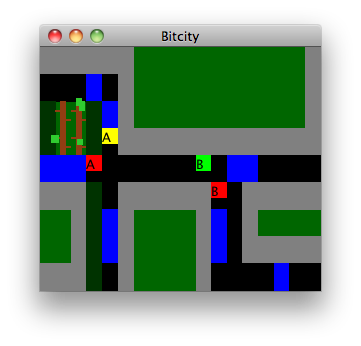
\includegraphics[scale=0.58]{figs/map1_1.png}
  }
  \subfigure[Chovendo no mundo, carro com retângulo branco buzinando \label{fig2}]{
    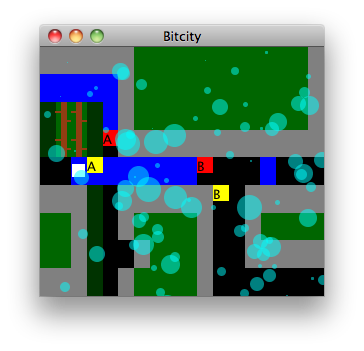
\includegraphics[scale=0.58]{figs/map1_2.png}
  }
  \caption{Modelo \ref{short-one} renderizado}
\end{figure}

A distinção entre ruas e vegetação comum exibida não requer elementos
especiais no modelo textual. O algoritmo \textit{4-way flood fill} é
aplicado a um ponto de partida qualquer e todas as posições atingidas,
considerando que calçada, garagem e vegetação rasteira são bordas
nesse preenchimento, são coloridas de preto. Isso colore todas as ruas
devido a restrição dos pontos serem ligados. Em relação a calçadas e
estacionamentos, atualmente não há distinção visual entre os dois
elementos.

A renderização do mundo ocorre em um \textit{thread} a parte, sendo
esta criada durante a inicialização da aplicação. É permitido ajustar
a velocidade da taxa de atualização, ou \textit{Frames Per Second} (FPS),
durante a execução, podendo variar de 30 a 45 renderizações por
segundo do mundo por completo. Durante estas atualizações também
decide-se entre criar um novo carro (classe \verb!Car!) ou não,
inserir uma ambulância ou não, iniciar chuva e também brotar folhas em
árvores.

Além da \textit{thread} principal e da \textit{thread} para desenho,
cada instância de classes que tem como pai a \verb!WorldObject! também
é uma \textit{thread}. Isso inclui todos os veículos que vão sendo
criados, todas as árvores, os sinais de trânsito e chuva.

A sincronização entre semáforos de um mesmo grupo deve ser realizada
para garantir que apenas um deles permaneça aberto durante um período
de tempo, eliminando a ocorrência de acidentes neste mundo ideal. Para
cada letra encontrada no modelo, uma instância da classe
\verb!TrafficLight! é criada e cada um destes recebe uma instância da
classe \verb!Semaphore! que controla os estados de um sinal de
trânsito. Isso é realizado de forma que um mesmo conjunto de letras
receba a mesma instância de um \verb!Semaphore! e, juntamente com a
\textit{keyword} \verb!synchronized! da linguagem Java, assim,
consegue-se limitar o acesso ao método \verb!Semaphore.open! a uma
única instância de um dado conjunto de \verb!TrafficLight!.

Também é feito uso do recurso de sincronização fornecido pela
\verb!synchronized! para avisar (ou alertar) a instância da classe
\verb!Rain! quando deve-se iniciar a chuva. Esse controle é feito da
seguinte forma: ao iniciar a \textit{thread} de \verb!Rain!, ela
invoca o método \verb!Thread.wait! com sincronização no objeto da
instância e, durante a execução da aplicação, a \textit{thread} de
\verb!WorldMap! sincroniza com o mesmo objeto mas faz uso do método
\verb!Thread.notify! para comunicar a \textit{thread} de \verb!Rain!
que esta deve começar a fazer chover. A determinação de quando o
método \verb!Thread.notify! é de fato chamado depende do sorteio de
números aleatórios e também da satisfação da condição de já não estar
chovendo.

Um último recurso de destaque no mundo é a ambulância, criada por meio
da classe \verb!Ambulance!. É permitido que somente uma desta esteja
no mundo ao mesmo tempo e ela só é criada caso o total de carros em
circulação seja superior a quantidade $max - 4$. Uma ambulância age
como uma forma de coletor de \textit{threads}, destruindo carros que
estejam em seu caminho e que não se desloquem ao mesmo tempo em que a
ambulância passa. Isso é feito pois a criação de linhas de execução
extras consome espaço no \textit{heap}, sendo possível ultrapassar o
limite disponível com mapas maiores que comportam uma grande
quantidade de carros ao mesmo tempo.% XXX Falar ainda do problema que
%isso vai causar XXX. XXX Colocar alguma referencia em relação ao
%tamanho variável que uma thread pode ocupar em heap quando criada XXX.

A remoção de veículos no mundo ocorre por meio do uso de exceções. No
momento em que um carro toma a decisão de sair do mundo, uma exceção é
levantada e o método \verb!run! do respectivo objetivo trata essa
situação como encerramento da \textit{thread}. No caso de ambulância
também é feito uso da \textit{keyword} \verb!finally! para garantir
que um efeito sonoro, que é iniciado ao instanciar uma ambulância,
seja desativado. Em outros momentos onde ocorre a utilização de
efeitos sonoros, também é feito uso de tratamento de exceções para
garantir que problemas de: falta de suporte ao formato de audio,
arquivo inexistente ou dispositivo de som ocupado; não causem um
encerramento prematura da aplicação.

\section{Hierarquia de Classes}

A Figura \ref{hierarchy} apresenta a hierarquia das classes da
\textbf{Bitcity}.

\begin{figure}[ht!]
  \centering
  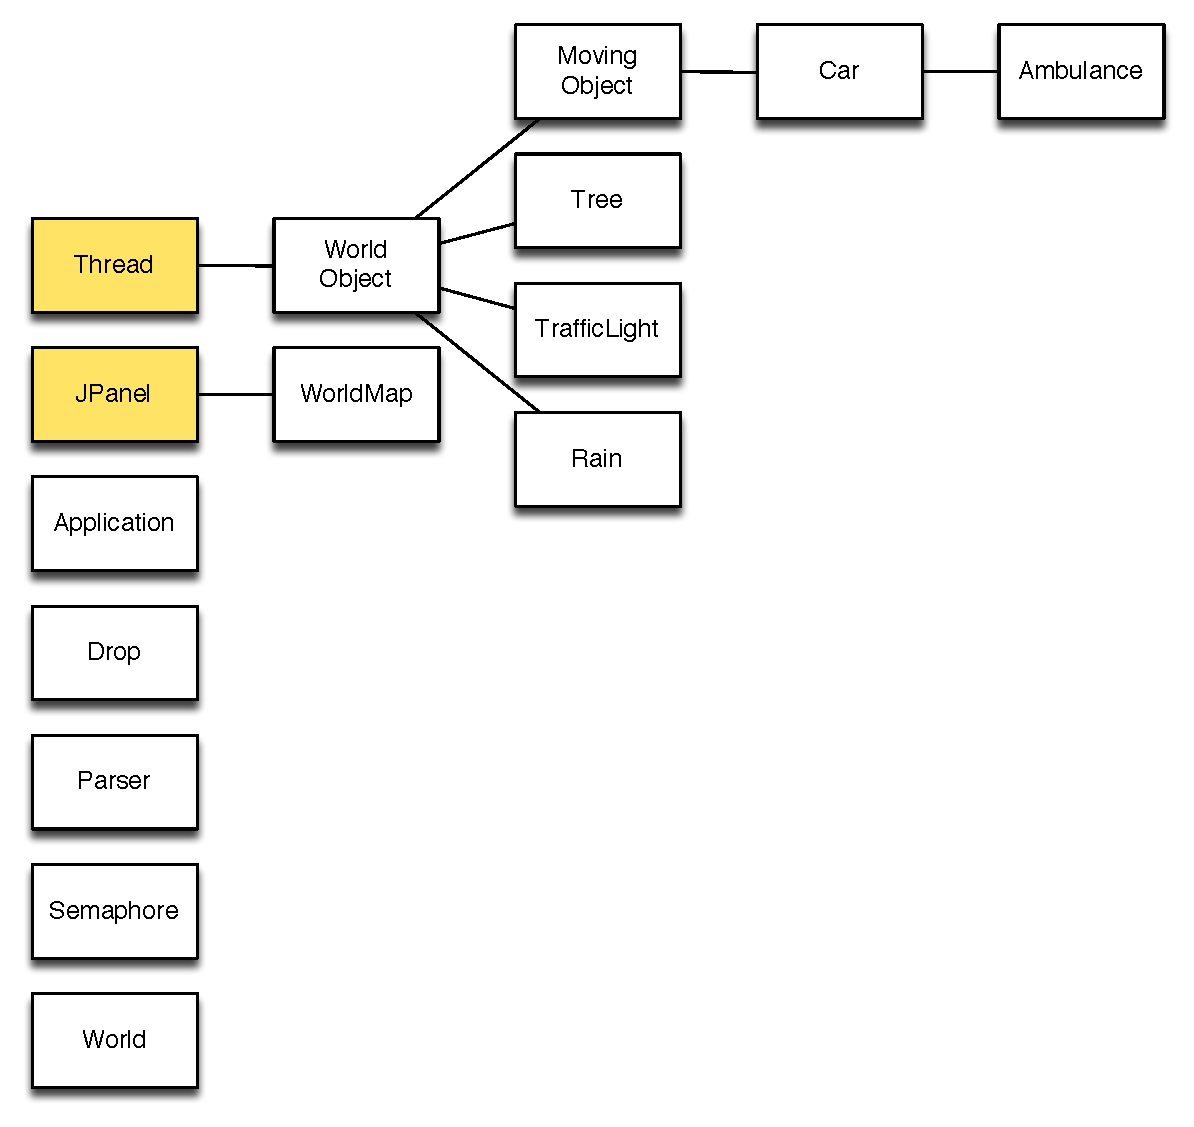
\includegraphics[scale=0.58]{figs/hierarchy}
  \caption{Classes em amarelo percentem a Java, em branco a aplicação \label{hierarchy}}
\end{figure}

A classe \verb!Application! ficou responsável por implementar o método
\verb!main! e iniciar a execução da aplicação. A classe \verb!Drop! é
utilizada pela \verb!Rain! para desenhar as gotas de chuva. Por
último, a \verb!TrafficLight! faz uso da \verb!Semaphore! para
controlar o tráfego.

\chapter{Conclusão}
\label{chap:conclusao}

1 página (+/- o limite)


\bibliographystyle{anbt-alfheng}
\bibliography{biblio}

\pagebreak

\end{document}
